%!TEX root = report.tex
\section{Generating Reference Timetable}
\label{sec: official_tfl_timetable}
For each day of the week, there are a predefined number of running the give route. We used the \texttt{VehicleJourneys} as a starting point to retrieve the departure time of the actual vehicle from the terminal. We then retrieved the corresponding \texttt{JourneyPattern}, and obtained the travel time between each neighbouring stops on the route for the given vehicle journey, to compute the cumulative travel times throughout the route.

The above computation was performed on each XML file to generate the actual arrival time and travel time for each vehicle trip at each stop in the route throughout the day. We grouped the bus travel time by the hour that the arrival time falls in, and find the average bus travel time between every pair of the neighbouring stops for the given hour of the given day of the week. The results of this computation was stored in the \texttt{delay\_tfl\_timetable} table (Table \ref{table:delay_tfl_timetable}).

\subsection{Detailed Steps}

\par We used the \texttt{ElementTree} XML API in Python \cite{elementtree} to extract the official bus travel times between stops from the Journey Planner Bus Timetables\cite{open_data_feeds_description}. Each \acrshort{xml} file contains bus schedule information for one route. We carried out the following steps on each \acrshort{xml} file. To make the steps easier to understand, we took the first bus for route C2 on Saturday morning for example, and included figures of the relevant XML snippets to extract bus travel times.

\begin{figure}
\centering
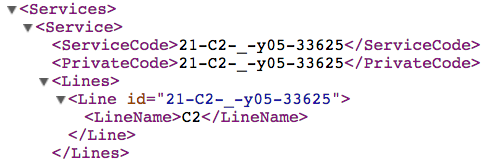
\includegraphics[width=\textwidth]{figures/xml_linename.png}
\caption{\label{fig:xml_linename} TfL Journey Planner Timetables XML LineName}
\end{figure}

\begin{figure}
\centering
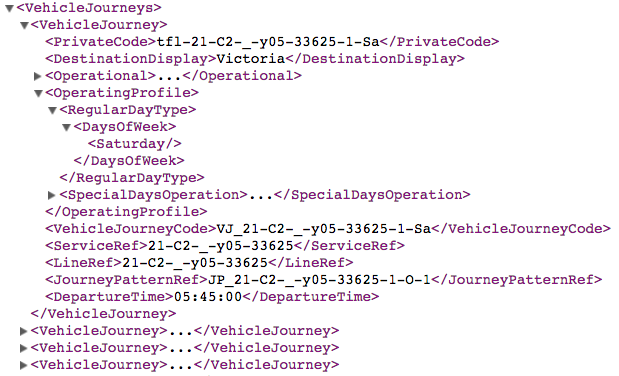
\includegraphics[width=\textwidth]{figures/xml_vehicle_journeys.png}
\caption{\label{fig:xml_vehicle_journeys} TfL Journey Planner Timetables XML VehicleJourney}
\end{figure}


\begin{figure}
\centering
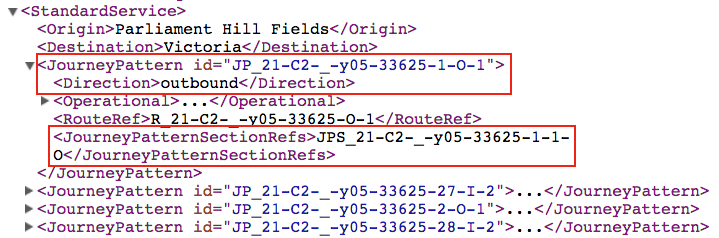
\includegraphics[width=\textwidth]{figures/xml_journeypattern.png}
\caption{\label{fig:xml_journeypattern} TfL Journey Planner Timetables XML JourneyPattern}
\end{figure}

\begin{figure}
\centering
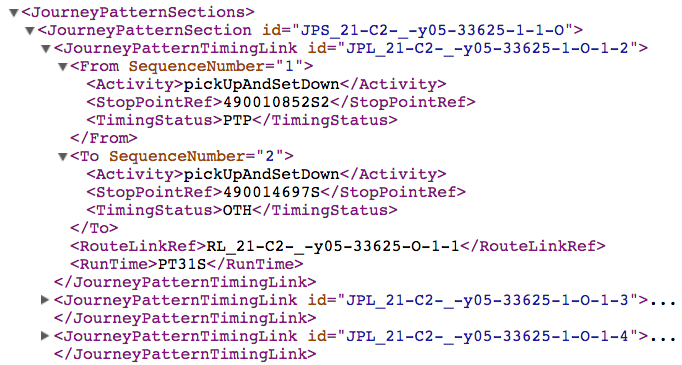
\includegraphics[width=\textwidth]{figures/xml_journey_pattern_section.png}
\caption{\label{fig:xml_journey_pattern_section} TfL Journey Planner Timetables XML JourneyPatternSection}
\end{figure}

\begin{figure}
\centering
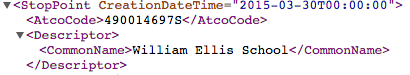
\includegraphics[width=\textwidth]{figures/xml_stoppoint.png}
\caption{\label{fig:xml_stoppoint} TfL Journey Planner Timetables XML StopPoint}
\end{figure}

\begin{enumerate}
  \item Obtain the route from \texttt{Services} $\rightarrow$ \texttt{Service} $\rightarrow$ \texttt{Lines} $\rightarrow$ \texttt{Line} $\rightarrow$ \texttt{LineName}, \textit{C2}. (Figure \ref{fig:xml_linename})
  \item For each \texttt{VehicleJourneys} $\rightarrow$ \texttt{VehicleJourney} (Figure \ref{fig:xml_vehicle_journeys}), extract the followings:
  \begin{enumerate}
    \item The departure time from \texttt{DepartureTime}, \textit{05:45:00}.
    \item The days of the week that this journey operates on from \texttt{OperatingProfile} $\rightarrow$ \texttt{RegularDayType} $\rightarrow$ \texttt{DaysOfWeek}, \textit{Saturday}.
    \item The corresponding journey pattern reference from \texttt{JourneyPatternRef}, \textit{JP\_21-C2-\_-y05-33625-1-O-1}.
  \end{enumerate}
  \item Each \texttt{JourneyPatternRef} maps to one Journey Pattern Section. This mapping is stored in \texttt{Services} $\rightarrow$ \texttt{Service} $\rightarrow$ \texttt{StandardService} $\rightarrow$ \texttt{JourneyPattern} (Figure \ref{fig:xml_journeypattern}).

  Retrieve the corresponding Journey Pattern Section Reference as such:
    \begin{enumerate}
      \item Each \texttt{JourneyPattern} element contains an element id, and a sub-element \texttt{JourneyPatternSectionRefs}.
      \item Map each Journey Pattern id to its corresponding \\ \texttt{JourneyPatternSectionRefs} for reference.
      \item Consult the above mapping to retrieve the Journey Pattern Section Reference for each Journey Pattern Reference found in Step 2(c). In the example case shown in Figure \ref{fig:xml_journeypattern}, \texttt{JourneyPattern} with \texttt{id=}\textit{JP\_21-C2-\_-y05-33625-1-O-1} has \texttt{JourneyPatternSectionRefs} \textit{JPS\_21-C2-\_-y05-33625-1-1-O}.
      \item Obtain the direction from the \texttt{Direction} sub-element. After comparing with the \acrshort{tfl} Bus Sequences data, we found out that \texttt{outbound} corresponds to run 1 and \texttt{inbound} corresponds to run 2.
    \end{enumerate}
    \item Next, obtain the bus travel time between every pair of neighbouring stops in the route from the \texttt{JourneyPatternSections} (Figure \ref{fig:xml_journey_pattern_section}). The detailed steps are as the following:
    \begin{enumerate}
      \item For each \texttt{JourneyPatternSectionRefs}, find the corresponding \texttt{JourneyPatternSections} $\rightarrow$ \texttt{JourneyPatternSection} with the same id, \textit{JPS\_21-C2-\_-y05-33625-1-1-O}.
      \item Each \texttt{JourneyPatternSection} contains multiple \\ \texttt{JourneyPatternTimingLink} sub-elements. Each sub-element contains information for one pair of neighbouring bus stops. Retrieve the following information from each sub-element:
      \begin{enumerate}
        \item \texttt{From SequenceNumber}, \textit{1}.
        \item \texttt{From} $\rightarrow$ \texttt{StopPointRef}, \textit{490010852S2}.
        \item \texttt{To SequenceNumber}, \textit{2}.
        \item \texttt{To} $\rightarrow$ \texttt{StopPointRef}, \textit{490014697S}.
        \item \texttt{RunTime}, \textit{31 seconds}.
      \end{enumerate}
    \end{enumerate}
    \item Each \texttt{StopPointRef} maps to a \texttt{StopPoints} $\rightarrow$ \texttt{StopPoint} $\rightarrow$ \texttt{AtcoCode} element. Each \texttt{StopPoint} element contains the stop name in its \texttt{Descriptor} element (Figure \ref{fig:xml_stoppoint}).

    For each \texttt{StopPointRef} obtained in step 4(b), retrieve the corresponding stop name as such:
    \begin{enumerate}
      \item Go through every \texttt{StopPoint} to build a map from \texttt{AtcoCode} to \texttt{Descriptor}.
      \item Consult the above mapping to retrieve the stop name for each \texttt{StopPointRef} found in step 4(b), \textit{William Ellis School}.
    \end{enumerate}

    \item After performing the above steps for every data point, we would have obtained the departure time from the terminal stop for each vehicle journey (Step 2(a)), and the bus travel time between every pair of the neighbouring stops (Step 4(b)v.). We calculated the cumulative bus travel time for each stop, and derived the bus arrival time at each stop for the given vehicle journey. We included a column \texttt{arrival\_hour} to store the hour that the arrival time falls in. This data is stored in the \texttt{delay\_tfl\_timetable\_archive} table. Figure \ref{fig:tfl_timetable_archive_sample} shows some sample entries from this table returned by the following SQL query.

    \begin{verbatim}
SELECT route, day, run, sequence, stop_name,
       naptan_atco, departure_time_from_origin,
       travel_time, cumulative_travel_time,
       arrival_time
FROM delay_tfl_timetable_archive
WHERE route='C2' AND day='Saturday'
      AND arrival_hour = 5 AND run = 1
ORDER BY sequence, departure_time_from_origin
    \end{verbatim}

\begin{figure}
\centering
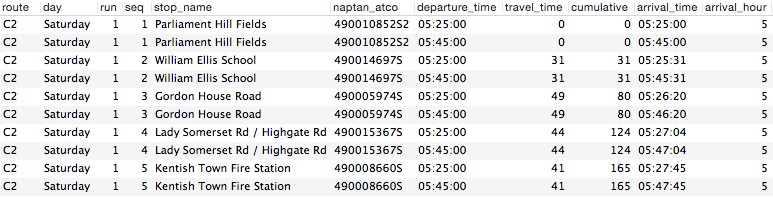
\includegraphics[width=\textwidth]{figures/tfl_timetable_archive_sample.png}
\caption{\label{fig:tfl_timetable_archive_sample} TfL Timetables Archive Sample}
\end{figure}

    \item As the \texttt{delay\_tfl\_timetable\_archive} table has more than 12 million entries, it was slow to run queries on it. Response time could go up to more than 20 seconds. In order to improve query performance, we further grouped the entries by \texttt{arrival\_hour}, and computed the average bus travel time between every pair of the neighbouring stops for the given hour of the given day of the week. This data was stored in the \texttt{delay\_tfl\_timetable} table (Schema shown in Table \ref{table:delay_tfl_timetable}) by running the following SQL statement. The resulting table has about 2.8 million entries and a query response time of about 5 seconds.

\begin{verbatim}
INSERT INTO delay_tfl_timetable
(route, day, run, sequence, stop_name,
naptan_atco, average_travel_time, arrival_hour)
(SELECT route, day, run, sequence, stop_name, naptan_atco,
        AVG(travel_time) as average_travel_time, arrival_hour
 FROM delay_tfl_timetable
 GROUP BY route, day, run, sequence, arrival_hour)
\end{verbatim}

    Figure \ref{fig:tfl_timetable_sample} shows sample average travel times for route C2 outbound journeys on Saturday morning 5am. We observed that there are less number of entries than the sample shown in Figure \ref{fig:tfl_timetable_archive_sample}.

\begin{figure}
\centering
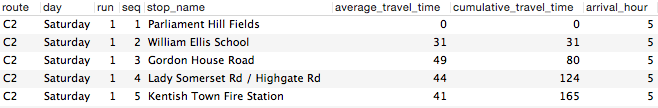
\includegraphics[width=\textwidth]{figures/delay_tfl_timetable_sample.png}
\caption{\label{fig:tfl_timetable_sample} TfL Timetables Sample}
\end{figure}

\end{enumerate}

The \acrshort{tfl} Reference Timetable is thus generated.



